\documentclass{article}


% Language setting
% Replace `english' with e.g. `spanish' to change the document language
\usepackage[english]{babel}
% Set page size and margins
% Replace `letterpaper' with `a4paper' for UK/EU standard size
\usepackage[letterpaper,top=2cm,bottom=2cm,left=3cm,right=3cm,marginparwidth=1.75cm]{geometry}
% Useful packages
\usepackage{amsmath}
\usepackage{graphicx}
\usepackage[colorlinks=false, allcolors=blue]{hyperref}


\title{Exploring Scope of Applying Deep Learning Techniques on 3D Agriculture Data}
\author{Ashish Rana, 1822317 \\
        ashish.rana@students.uni-mannheim.de}


\begin{document}
\maketitle
\tableofcontents % table of content
% \listoftables % list of table added
\newpage


\begin{abstract}


Modern day agriculture is responsible for 70 \% percent of water consumption needs globally.
Growing certain opulent products like almonds, avocados, and apples, disproportionately consumes huge volumes of water which further strains the local water resources.
Modern computer vision approaches have shown promising results for improving growth efficiency of these fruits by monitoring their counts, sizes, and exact growth cycles at large scale.
This manuscript theoretically explores modern deep learning architectures that detect, count, and segment Fuji apples across 2D images and 3D point cloud data modalities.
Second, we analyze the scope of applying point cloud convolutional architectures directly on 3D point clouds to analyze large agriculture fields.
Finally, in experiments we present the results and challenges of applying deep learning models on point clouds for segmentation on large agricultural datasets.
The code repository implementation is present at \href{https://github.com/arana-initiatives/agro-point-cloud-seg-pipeline}{github.com/arana-initiatives/agro-point-cloud-seg-pipeline}.


\end{abstract}


\section{Introduction}


For sustainable agriculture which minimizes the negative environmental impact there is a need to develop newer innovative agricultural methods that benefit everyone from farmers, to consumers, and to nature.
Proper intake of fruits and vegetables helps in avoiding serious diseases, and lots of opulent fruits, like almond, apples, avocados etc. strongly helps in maintaining a healthy disease free body.
But, these fruits like Fuji apples \textit{(Malus domestica Borkh. cv. Fuji)} consumes a very high amount of water resources which puts the nearby water bodies under pressure.
In longer run through precision agriculture more effective in field fruit monitoring is required to optimize the fruit-growth management tasks.
Image processing techniques have proved to be effective tools for building modern effective farming systems. 
For an effective fruit plantation cycle these systems can determine fruit location, fruit size, visible fruit and tree diseases, airflow through the orchards, and irrigation routes etc. \cite{fu2020application, koirala2019deep}
These techniques by providing more precise insights helps farmers to increase their crop yield, and reduce resource costs.
These innovations in computing technologies additionally give secondary benefits, like longer maintain soil quality, minimal water usage, and better supply-chain management cycles.
These multifaceted benefits provide favorable arguments for all the more reasons to invest in such technologies.


Knowledge of spatial information \textit{(3D)} is of high interest value because it allows the farmers to have better harvest and production estimates, which further leads to better storage, harvesting, and marketing \cite{bargoti2017image}.
Most commonly used sensors involve RGB, spectral, and hyperspectral cameras, as well as for spatial data LiDAR \textit{(Light Detection and Ranging)} and RGB-D cameras.
Practically, with decreasing sensor prices even thermal cameras with RGB-D depth estimation have been utilized for in field fruit size estimations for fruits like apples, mangoes, oranges, and grapes \cite{stajnko2004estimation}. 
The standard RGB cameras are the cheapest monitoring resource but object occlusions are a real challenge, and incorporating multiple camera sensors increases the total monitoring cost.
Additionally, environmental factors, like sun orientation, rain etc. also play an important role in determining quality of data acquired by RGB, RGB-D, and thermal cameras.
The 3D representations from LiDAR sensors can give high fidelity spatial data but these sensors are quite expensive and are not user-friendly as well.
But, methods like structure-from-motion (SfM) techniques can also give good 3D representations with multiple cheap camera sensors deployed across different orientations.
The 3D data analysis does easily overcome issues caused because of occlusions, unstructured crops, and bad lighting conditions but does introduce its own complexity set. 


The 3D point cloud segmentation classifies point clouds in homogeneous regions where similar regional points have the same properties.
The solutions to this problem have propelled domains like robotics and navigation to achieve new milestones.
But, processing agricultural 3D data can be especially challenging considering the scale, and associated complexity with different crops.
Here, we focus on proposing deep learning solutions that meet the theoretical feasibility threshold of being utilized as 3D point cloud processing systems for fruits.


In this manuscript, we first discuss some of the previous work related to usage of vision algorithms for agriculture, and previously used relevant ideas for point cloud data processing.
Second, in two separate sections we discuss 3D point cloud data processing for agriculture datasets, and current deep learning landscape against standard benchmarks.
Third, we discuss and propose our solution to process point clouds of agriculture datasets with deep learning based systems.
Finally, we conclude our exploration study and practically quantify the scope of such application with small experimentation \footnote{ Experimentation code available at the repository \href{https://github.com/arana-initiatives/agro-point-cloud-seg-pipeline}{github.com/arana-initiatives/agro-point-cloud-seg-pipeline}.}.


\section{Previous Work}


Previously, for agricultural data processing plathero of traditional approaches have been developed to measure fruit yield, count, and geometries \cite{syal2013survey}.
For example, for recognizing fruit shapes a KNN algorithm that classifies fruits based on mean color values, area and perimeter has shown good results for 2D images when combined with the circle fitting algorithm \cite{seng2009new}.
Furthermore, for fruit location estimation traditional machine learning combined with efficient feature extraction modules which calculates color, intensity, orientation, and fruit edges have achieved 90 \% accuracy on 2D images in the past \cite{patel2011fruit}.
Finally, multiple other approaches have been analyzed which explore the influence of different image properties and data acquisition methods on multimodal agricultural use-cases \cite{jimenez2000survey}.


Parallely, lots of approaches that analyze point clouds as meshes, and voxels etc. have also developed over the years \cite{nguyen20133d}.
For example, VV-Net converts the point cloud into more structured voxels and uses kernel-based interpolated variational autoencoders for encoding the local geometry \cite{meng2019vv}.
Second, OctNet uses the sparsity of data to generate unbalanced octrees to directly apply OctNet 3D convolutional operation on the different size partitions to generate richer representations by focusing more on dense node regions \cite{riegler2017octnet}.
The segmentation task is especially challenging in general because it has very high redundancy, uneven density, and lacks structural properties.
Essentially meaning, the above discussed approaches lose fidelity in their learnt representations when they transform the point cloud into other relatively simpler structures.
Therefore, applying such approaches on realistic agriculture point cloud data will definitely give lower performance results.
Further down in this manuscript, we discuss and elaborate the modern deep learning architectures that inputs the unstructured point cloud data and directly apply convolution operations on it.


\section{3D Data Analysis Approaches in Agriculture Use-Cases}


This section explores the current advancements in 3D data processing and innovative use-cases being developed in the modern agriculture space.
In below subsections we explore the relevant datasets for analyzing Fuji apple growth parameters, and the corresponding approaches in use to analyze two of those datasets.
We also explore the quantitative advantages and limitations of using those approaches in relevance to point cloud data processing.


\subsection{Description of Agriculture Datasets}


Several datasets have been developed by the GRAP group from University of Lleida, Spain to explore different properties of Fuji orchards to further supplement the existing agriculture techniques with modern data insights.
Here, they have used traditional cameras, LiDAR sensing, and Microsoft Kinect v2 etc. to generate different data modalities, like 2D images, 2D RGB-D images, and 3D point clouds etc.
These datasets help in analyzing a plethora of aspects with respect to Fuji orchards, like fruit location detection, diameter estimation, yield prediction, several growth and geometric characterizations.
Below, we provide a basic description of a few of these Fuji apple datasets, and finally elaborate more on \textit{PFuji-Size} and \textit{Fuji-SfM} to further analyze their data processing methodologies.


\begin{figure}[h]
    \centering
    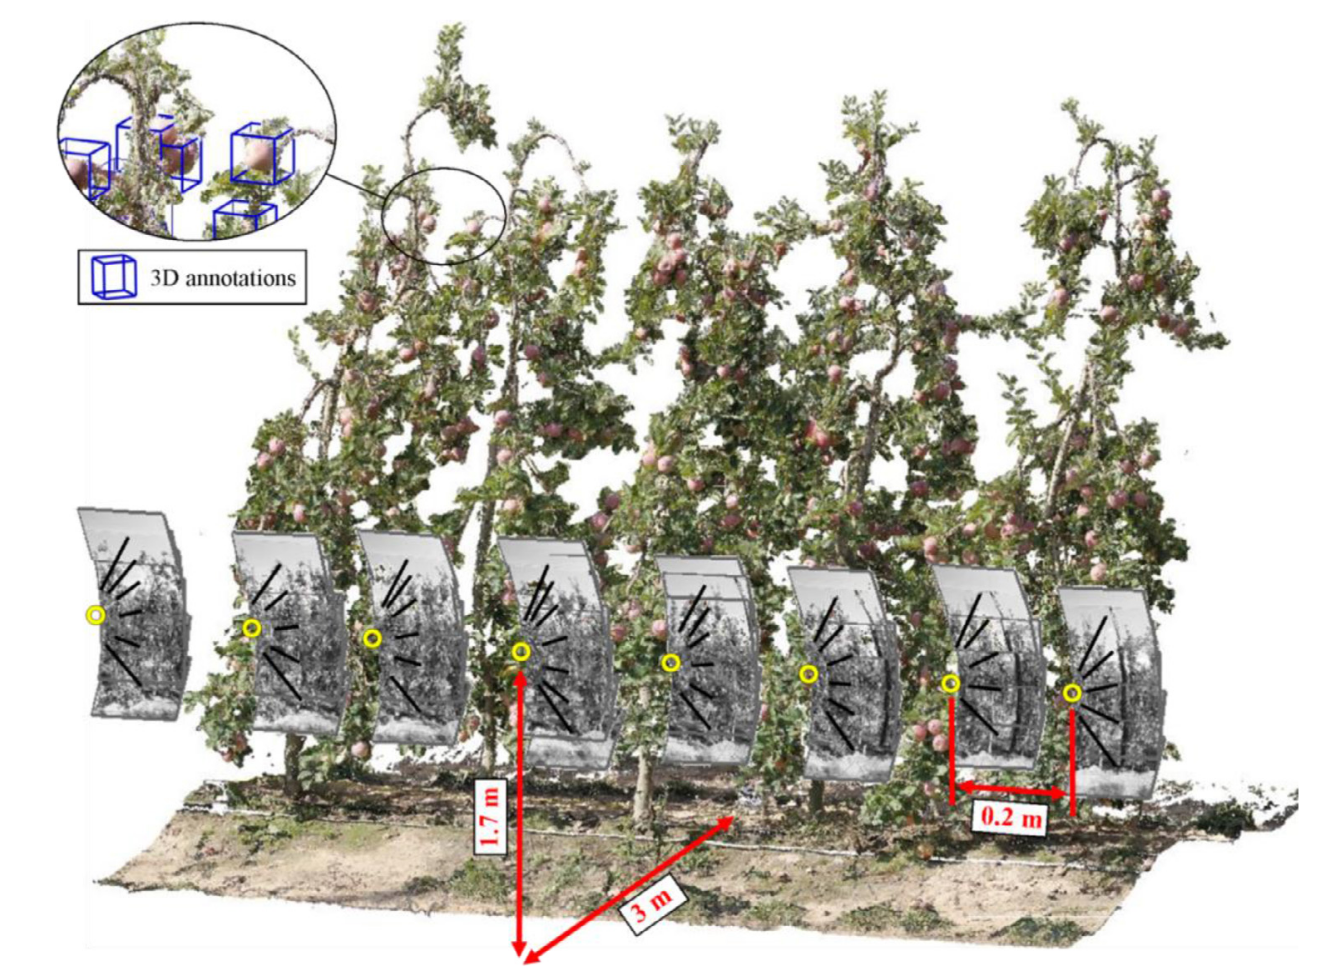
\includegraphics[width=0.65\textwidth]{fuji-sfm-dataset.png}
    \caption{The isometric view of scanned Fuji apple trees where yellow circles represent photographic positions and 3D blue cuboids represent bounding box annotations for apples. \textit{(Image Credit: Gen{\'e}-Mola et al.)}}
    \label{fig:fuji-sfm}
\end{figure}


The \textit{AgLiMatch dataset} provides LiDAR data captures and Global navigation satellite system (GNSS) tracks using an autonomous platform robot of the Fuji apple orchard to analyze optimum movements in agricultural lands.
This dataset was used to compare optimum robot navigation paths generated from LiDAR scans and actual platform path ground truth measured with GNSS \cite{guevara2021comparison}.
The \textit{KEvOr dataset} uses three Microsoft Kinect v2 sensors to scan Fuji apple trees under different illuminations and generate RGB-D image outputs. These images were further used to characterize tree canopies under different lighting conditions \cite{gene2020assessing}.
The \textit{LFuji-air dataset} provides scans of 11 Fuji trees with different sensor positions and forced airflow conditions which allows airflow analysis across the orchard alongside measurement of standard fruit yield related metrics \cite{gene2020lfuji}.
The point cloud data obtained from this dataset was further used to detect fruits, estimate yield, and geometrical categorization canopies \cite{gene2020fruit}.
The \textit{KFuji RGB-DS database} was designed for reliable detection and localization of fruits to yield high-value Fuji apple crops.
In this dataset Microsoft Kinect v2 was used to measure RGB \textit{(color)},  D \textit{(color)}, and S \textit{(reflectance)} to generate multi-modal images \cite{gene2019kfuji}.
This dataset was used to further design and develop novel deep learning systems which utilizes depth and reflectance channel information effectively \cite{gene2019multi}.


The \textit{Fuji-SfM} dataset contains 288 Fuji apple orchard segmented images for instance segmentation training, and 582 additional images in motion sequence for 3D model generation by structure-from-motion (SfM) photogrammetry \cite{gene2020fuji}.
Further, this dataset provides a million order 3D point cloud with RGB channel information with manual bounding box annotations.
This dataset is designed to train models with either 2D images, 3D point cloud or multimodal inputs. 
The 3D model of 11 Fuji trees in the orchard was reconstructed by using the  SfM-set images as shown in Figure \ref{fig:fuji-sfm}.
And, the 3D point cloud for each tree row was generated based on bundle adjustment with multi-view SfM photogrammetry \cite{triggs2000bundle}.
The \textit{PFuji-Size dataset} contains 3D point clouds scanned from SfM and multi-view stereo (MVS) techniques capturing different maturity stages with 3D annotated apple point clouds \cite{gene2021pfuji}.
The data points are acquired at two different growth stages with west and east side scanning orientations to capture different illumination levels for the final generated point cloud.
This finally generated point cloud is then segmented spherically to generate apple point cloud annotations as shown in Figure \ref{fig:fuji-size}.
Practically, for applying 3D point cloud segmentation model this dataset provides more point cloud data points \textit{(10+ million order)} and more accurate apple class annotations but is not well documented for data preprocessing.


\begin{figure}[h]
    \centering
    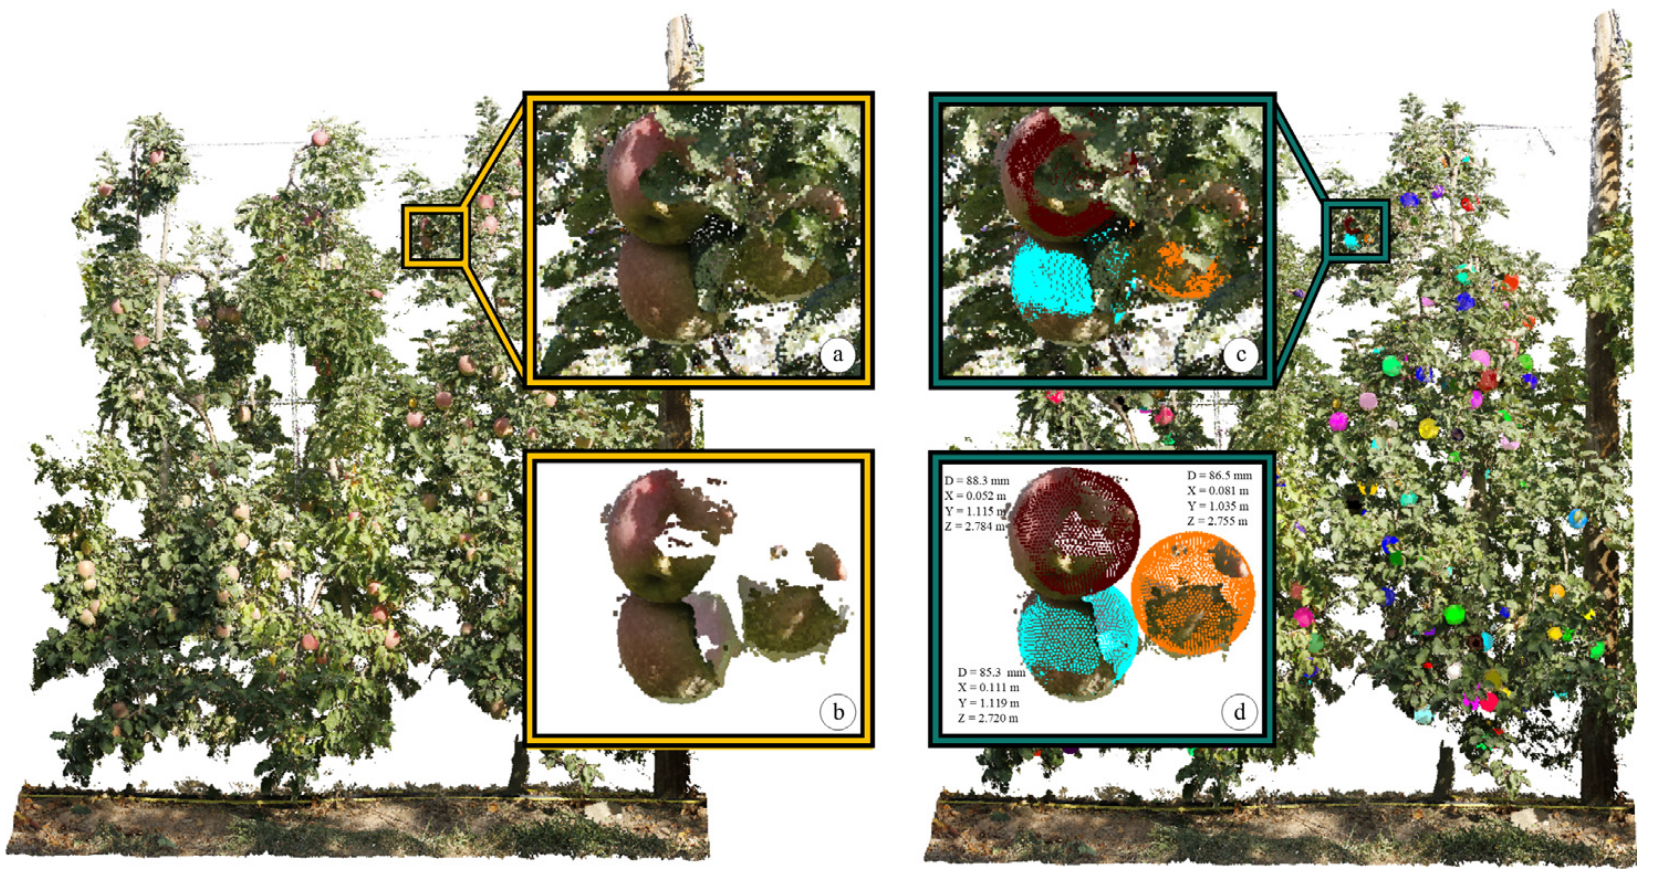
\includegraphics[width=0.85\textwidth]{pfuji-size-dataset.png}
    \caption{The spherical point cloud annotations for the apples provided in the \textit{PFuji-Size dataset}, where (a) represents the complete point cloud, (b) represents the segmented apples without background, (c) represents ground truth for apple annotations, and (d) specify the diameter with [X, Y, Z] coordinates of the apple centers. \textit{(Image Credit: Gen{\'e}-Mola et al.)}}
    \label{fig:fuji-size}
\end{figure}


\subsection{Data Processing Approach Description and Analysis}


First, we discuss the Mask R-CNN \textit{(Region-Based Convolutional Neural Network)} detection and segmentation networks on 2D images from \textit{Fuji-SfM} dataset, and utilization of projection of 2D images onto 3D dataset generated from SfM \cite{he2017mask, gene2020fruit}.
This approach obtains a F1-score of 0.816 on 2D fruit detection and a F1-score 0.881 on 3D fruit localization tasks respectively.
The major advantage of using Mask R-CNN for the 2D fruit detection task is its lower false positive rate and higher decision rate in this scenario.
But, the large processing time required for 3D data projection processing is a major bottleneck for this approach.


The original images encompasses a large number of apples which decreases the CNNs performance while predicting for small apple class objects.
Therefore, before training the instance segmentation model each image is split into 24 sub-images of 1024$\times$1024 pixels.
Further, these masked images are used to generate 3D models by using SfM, and camera alignment metrics are further used to project 2D detections onto these 3D point cloud data models. 
The Figure \ref{fig:fuji-sfm-pipeline} highlights the detection and projection pipeline to visualize the detected apples in 3D space under isolation without the background orchard trees.


\begin{figure}[h]
    \centering
    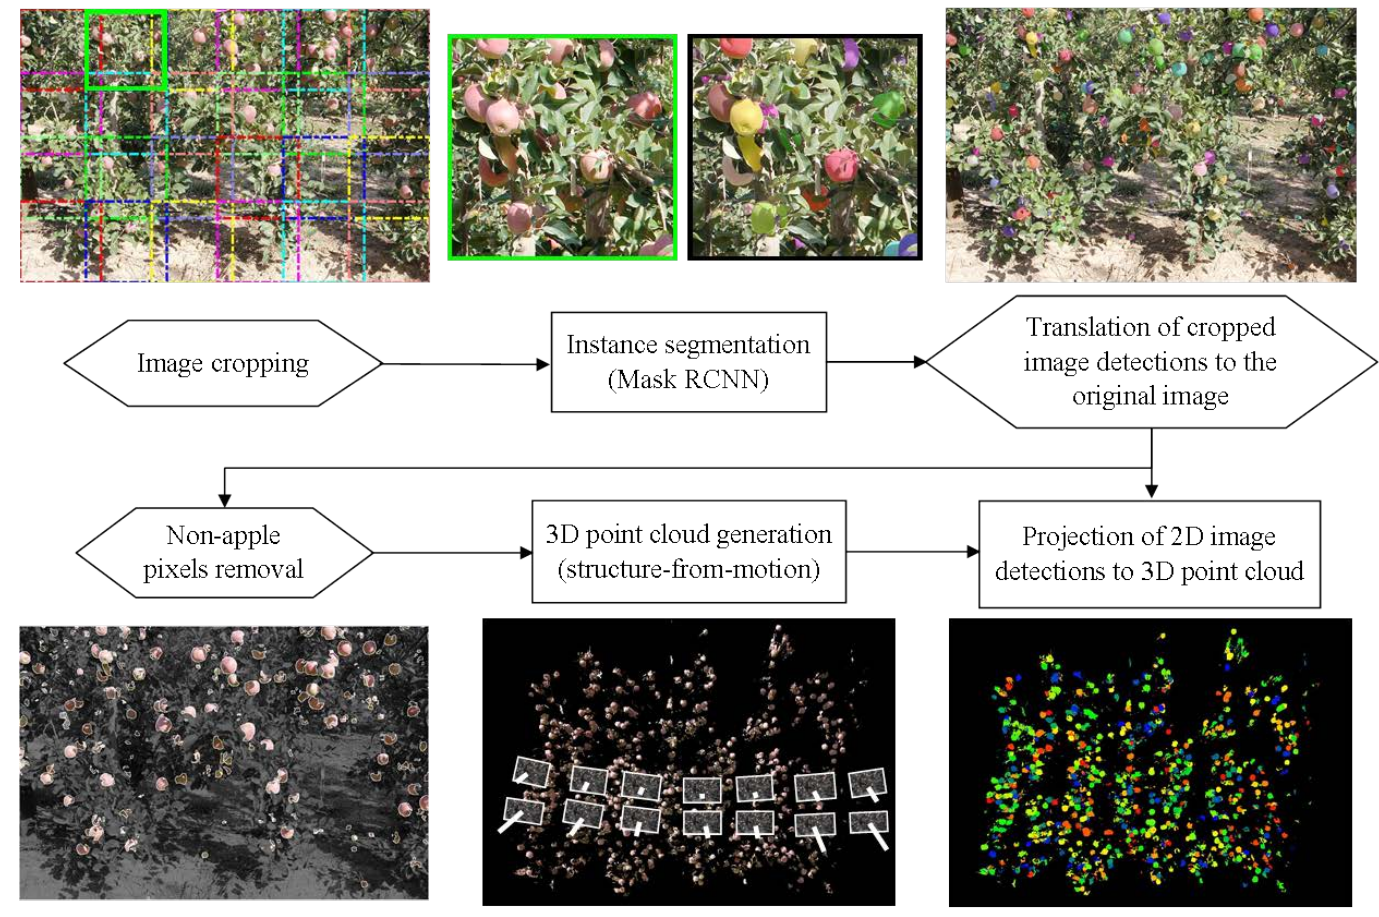
\includegraphics[width=0.65\textwidth]{fuji-sfm-pipeline.png}
    \caption{The Fuji apple detection and localization pipeline, where hexagons represent the data preparation steps and rectangles highlight the processing steps. \textit{(Image Credit: Gen{\'e}-Mola et al.)}}
    \label{fig:fuji-sfm-pipeline}
\end{figure}


The Mask R-CNN network consists of a backbone for feature extraction, a feature head for bounding box recognition and mask prediction, which is applied separately to each ROI \textit{(region of interest)}.
For training, ResNet-101-FPN backbone is used which uses FPN \textit{(Feature Pyramid Network)} architecture pre-trained on COCO dataset for Mask R-CNN with learning rate 0.001, momentum 0.9, and weight decay 0.0001 \cite{lin2017feature, he2016identity, lin2014microsoft}.
Further, a proprietary software is used for 2D to 3D projections while generating the point cloud for apple localizations from the 2D images detections.
After this extremely slow projection step \textit{(4 hours)}, a density based scan algorithm (DBSCAN) is used to find the connected components for the point cloud apple localizations to count the Fuji apples with tuned parameters.
This experimentation study does extensively work with 3D data but only to apply the DBSCAN clustering algorithm to a very low density apple point cloud ignoring the complex background point cloud data.


The second study compares apple size estimation approaches after the fruit detection and 3D projection steps on a different size estimation \textit{PFuji-Size} dataset.
This study estimates the fruit size by fitting an equivalent sphere to the localized apple point cloud in the 3D space \cite{gene2021field}.
For this task traditional approaches like traditional least squares \textit{(LS)}, and M-estimator Sample Consensus \textit{(MSAC, an iterative registration RANSAC algorithm implementation)} are compared \cite{derpanis2010overview}.
Additionally, a different template matching \textit{(TM)} approach is also applied to fit the standard 3D apple model with varying diameters to match other comparative apple point cloud models.
All these three methods produces very low mean absolute errors \textit{(MAE)} of 4.5 mm, 3.7 mm and 4.2 mm, and very high coefficients of determination \textit{(R\textsuperscript{2})} scores of 0.88, 0.91 and 0.88, respectively.
Further, for visibility estimate task which measures the percentage of point cloud overlapping with the fitted sphere surface achieves the coefficient of determination \textit{(R\textsuperscript{2})} score of 0.92.
Essentially meaning that both the apple size estimates and visibility estimates after occlusion are highly accurate and reliable.


For this study, also like the previously discussed study on \textit{Fuji-SfM} dataset, 3D data processing is again the most expensive step.
And, most importantly this approach also again analyzes detected apples in isolation for size estimation without the background tree point cloud.
Both these approaches reduce the complexity by analyzing apple point clouds in isolation. But, add complexity to the pipeline with proprietary tools, and additional data processing steps.
These discussed studies in summary solves relatively easier and already well explored problems related to 3D point cloud processing, like point cloud registration, DBSCAN clustering etc.
This further limits the novelty of these studies with respect to applicability on realistic point cloud datasets where segmenting fruits at large scale automatically is the hardest task.
Whereas, in these studies segmentation step is either done on limited 2D image data or done manually which is quite cumbersome.


\section{3D Data Analysis Approaches on Benchmark Datasets}


Even though the previously discussed approaches use 3D point cloud data for different purposes like, monitoring different aspects related to Fuji apple fruit growth.
But, none of them directly apply point cloud segmentation on these above discussed datasets directly.
These approaches do not generate inference on 3D data without the additional post-processing steps, and also require utilization of proprietary softwares.
First, in the subsections below we discuss some relevant 3D point cloud data benchmarks and analyze the model performance of different architectures on these datasets.
Finally, we discuss the application scope of these deep learning segmentation approaches on large scale point cloud agriculture datasets.
This direct inference on 3D point cloud will simplify the analysis pipeline by removing usage of post-processing steps, intermediate 2D image representations, and proprietary tools.


\subsection{Description of Benchmark Datasets}


The basic \textit{ModelNet dataset} provides 3D CAD models of different shapes in point cloud form, and it consists of 6670 models across 161 model categories \cite{wu20153d}.
Second, the \textit{ShapeNet dataset} provides an annotated 3D CAD model repository of a large number of realistic objects containing 220K annotated models across 3,315 categories \cite{chang2015shapenet}.
But, the point cloud size for the shapes present in both these datasets is not considerably large, and there aren’t specific cases where the shapes overlap or touch other geometries.


The \textit{Semantic3D dataset} belongs to the class of realistic datasets, it comprises 15 train and 15 test point cloud samples of 10\textsuperscript{8} size.
The samples in this dataset covers 160$\times$240$\times$30 meters of real world space, and provides additional intensity information alongside RGB information \cite{hackel2017semantic3d}.
Further, the \textit{S3DIS dataset} also provides realistic point cloud scans of 10\textsuperscript{7} size for the 271 scanned rooms belonging to much larger 6 areas for segmentation \cite{armeni_cvpr16}.
Finally, the \textit{SemanticKITTI dataset} consists of 43K annotated LiDAR scans for 21 sequences where each point cloud scan is of 10\textsuperscript{5} size spanning over 160$\times$160$\times$20 meters in real world space \cite{behley2019semantickitti}.
But, all the above discussed datasets are nowhere near to the complexity of agriculture point cloud datasets which annotate countless leaves, soil textures, trunks and branches as background class.
Hence, making the semantic differentiation between instances belonging to different fruit and background classes much harder for the trained point cloud segmentation model.
Essentially meaning, that the trained model would not learn to segregate different background objects from one another well to further precisely segment the fruit class.


\subsection{Data Processing Approach Description and Analysis}


A more intuitive representation for humans of visual data is 3D data, which contains no grid structure and is permutation invariant.
So, directly applying traditional convolution operations is not possible on these datasets.
Additionally, there are three primary challenges associated with the analysis of point cloud datasets, namely: a.) redundancy, b.) scale, and c.) complexity \textit{(e.g. uneven density, no structure etc.)}.
For handling the redundancy of point cloud datasets we can adopt different sampling techniques for reducing the size of our input data more meaningfully. 
Further, this can even help our models to start their learning on simpler representations without losing much of representational fidelity.


Heuristic based sampling techniques like Farthest Point Sampling (FPS), Inverse Density Importance Sampling (IDIS), and Random Sampling (RS) can directly be applied to datasets under consideration.
The FPS approach has good coverage of complete point sets where it captures the farthest metric space points to successfully encapsulate small objects in the given point cloud.
But, with associated complexity \textit{O(N\textsuperscript{2})} complexity it is quite slow for sampling large point clouds. 
Whereas, IDIS which samples points based on the point cloud density does improve the complexity to \textit{O(N)} but it is still quite slow for building near real-time systems.
Finally, random sampling provides \textit{O(1)} complexity but it does not capture important trends in the final subsampled point cloud.
The learning based sampling approaches like Generator-based Sampling (GS), Continuous Relaxation based Sampling (CRS), and Policy Gradient based Sampling (PGS) does yield better subsampled point clouds than heuristic based sampling techniques but are especially ineffective for larger point cloud datasets.
Therefore,  a system that randomly selects data points from large point clouds and meaningfully retains the geometric information can serve as a good alternative for processing agriculture data.


Network architectures like PointNet and PointNet++ operating point cloud data are capable of performing standard computer vision tasks like object classification, part segmentation, and semantic scene parsing \cite{qi2017pointnet, qi2017pointnet++}.
Whereas the performance of these architectures can further be improved by better training methodologies as shown by PointNeXt architecture \cite{qian2022pointnext}.
Additionally, Stratified Transformer uses the transformer based self-attention supplemented with stratified point cloud key sampling to capture both global and local features to outperform above architectures \cite{lai2022stratified}.
But, above architectures even after introducing multiple novelties does not capture rotation invariant features which might cause problems in detecting asymmetric fruits rotated across multiple axes in the 3D coordinates system.
The network architectures, like Riconv, Riconv++, and RepSurf incorporate these geometrical properties into their architectures by designing rotation invariant convolution operations, and triangle meshes and umbrella curvature to capture local geometries respectively \cite{zhang2019rotation, zhang2022riconv++, ran2022surface}.
But, these architectures even with more meaningful generalization gains in terms of learning representation capacity, and truly understanding geometric properties of point clouds can only take a limited amount of point cloud data as input.
This limited input size does not address the scalability issue aspect of point cloud data analysis even though the complexity aspect is handled by these architectures to some extent.


\begin{figure}[h]
    \centering
    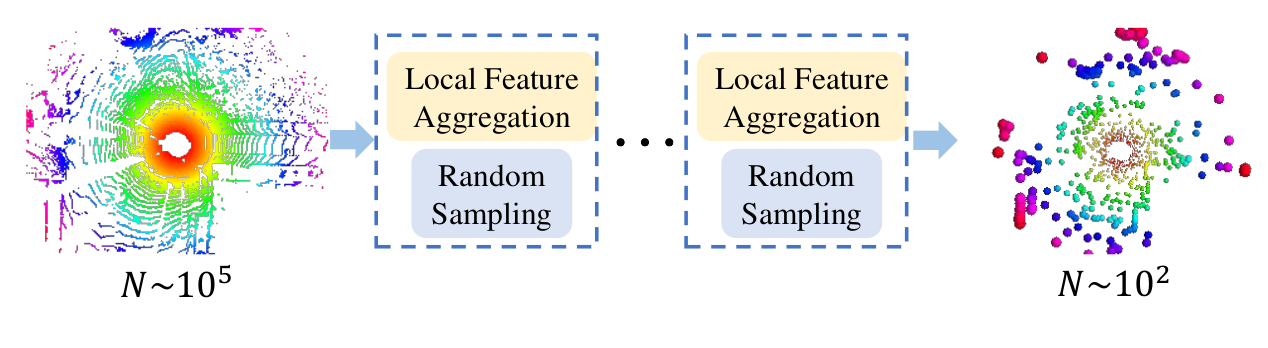
\includegraphics[width=0.65\textwidth]{randla-net-working.png}
    \caption{The qualitative functioning of RandLA-Net architecture for learning large representations of point cloud datasets. \textit{(Image Credit: Hu et al.)}}
    \label{fig:randla-net}
\end{figure}


The RandLA-Net model architecture attempts to mitigate all the above listed problems.
This architecture is capable of processing very large point cloud data inputs and also captures the point cloud complexity as well \cite{hu2020randla}.
The architecture achieves this by using consecutive local spatial encoding and attentive pooling blocks with dilated residual connections.
Essentially, this architecture contains a series of effective local feature aggregation, random sampling and attention modules, which carry out and learn an informed random sampling operation that attempts to capture all the important trends as shown in Figure \ref{fig:randla-net}.
This network demonstrates strong memorization capabilities and can predict for different object rotations provided similar multi-axes rotation samples are present during training.
Essentially, its geometry generalization capabilities are not equivalent to Rinconv++ and RepSurf architectures.
This network with good training methodologies and hyperparameter optimization achieves best trade-off between efficiency and effectiveness while designing real large scale point cloud systems.
All the above discussed architectures still haven’t been applied to agriculture datasets which comprises a much harder segmentation problem with a huge number of objects having limited differentiating annotations.


\section{Discussion}


With this manuscript we present several vision approaches from classical image processing to deep learning for determining fruit count, and size estimate. 
And, we also discuss the utilization of Mask R-CNN network for segmentation of Fuji apples, and projection approach to translate those masks into 3D point cloud space.
Second, we further explore the possibility of applying architectures like PointNet, PointNet++, and RandLA-Net etc. directly on the agricultural point cloud datasets.
In this subsection below, we state advantages and limitations of these discussed approaches in generality.


\subsection{Current Approach Advantages and Limitations}


With 2D image data either multi-channel or not there are several advantages and disadvantages for all data processing stages, like acquisition, pre-processing, model architectures, computation, and resources available.
During the data acquisition stage the quality of capturing device, lighting during capturing, and orientation of device strongly influences model performance. 
With higher quality, focused, and well lighted images the performance will be much better as compared to low resolution, badly lit, and object occluding images.
The resource availability and monitoring funding can strongly influence the above factors, and consistency in data acquisition for training is also important.
Additionally, segmentation architectures from YOLO series to Mask R-CNN are significantly fast and reliable as compared to point cloud segmentation models \cite{redmon2016you}.
But, 2D to 3D projection approaches based on multiple image scans, and highly occlusion of interest objects across image depth can lead to strong inconsistencies.
Further, analyzing data across multiple modalities makes the inference pipeline computationally complex adding several intensive processing steps.
Therefore, for use-cases requiring large scale analysis of fruit fields for more informative realistic 3D monitoring other options can be explored.


Similarly, 3D point cloud data either having RGB or normal feature information have several advantages and disadvantages for agriculture data processing.
3D data provides much higher accuracy of object geometry and relative positions in the realistic spatial domain.
With decreasing 3D sensing hardware technology prices it has become more feasible to utilize these alternatives for everyday usage.
Additionally, directly operating on point clouds simplifies the deep learning pipeline architecture eliminating all the post-processing steps required during 2D to 3D projection stages.
But, 3D data introduces its own set of challenges considering important parameters like scale, geometries, color information availability, sensor noise and occlusions of the point cloud data.
Although, these problems can affect the model performance in 2D images but for 3D point cloud data the performance degradation effect is more pronounced.


With point cloud data we can often only process a limited amount of input data with network architectures from PointNet to Transformers.
Therefore, sampling techniques also play an important role in generating meaningful downsampled representation of the point cloud.
Sampling techniques like FPS from PointNet++ produces good representations but adds additional computation complexity when compared with effective random sampling in RandLA-Net.
Additionally, most architectures do not capture geometric or rotational invariant features generalizations, like in RepSurf, Riconv, and Riconv++ networks.
But, rather display strong memorization capacity with respect to the different input data orientations.
With better training alternatives the problems like additional noise, missing RGB information, and geometry generalization can be mitigated as done in PointNeXt experimentation.
Instead, real challenging problems are training and inferencing for very large scale dense point clouds, and handling highly occluded objects from the scanner location.


A simple but not completely effective method for inference on large point clouds is to operate on smaller model architecture compatible patches but inference on the patch edges might be harder and might cause inconsistencies.
Second, for handling object occlusions multiple scanner locations can be used with overlapping point clouds which can further be merged with registration algorithms.
These registration algorithms add more complexity with additional preprocessing steps, and require scanner locations to be present at recommended locations.
But, when applied correctly these algorithms yield larger and more comprehensive point clouds with reduction in occluded object count.


\subsection{Possible Use-Case Application Pipeline}


The Figure \ref{fig:pipeline} describes a sample point cloud segmentation pipeline \footnote{ Experimentation code available at the repository \href{https://github.com/arana-initiatives/agro-point-cloud-seg-pipeline}{github.com/arana-initiatives/agro-point-cloud-seg-pipeline}.} for large agricultural datasets.
These highly practical datasets, unlike the datasets, introduce their own set of data acquisition limitations.
Like, changes in RGB information caused due to changing position of sun during the scanning process.
But, the segmentation models can still make good predictions with reasonable degree of accuracy without RGB features as well.
Hence, the primary problem for large 3D data processing is the limited availability of fruit point cloud data.
This causes high representational imbalance during model learning because the input point cloud will be further randomly subsampled and the fruit point cloud density will be further reduced.
Heuristic subsampling approaches like FPS, IDIS etc. can retain the fruit representation in the 3D space.
But, for efficiently processing million order point clouds the associated complexity is undesirable for near real-time inference.
Therefore, as described in the \textit{preprocessing} and \textit{generate patches} steps we reduce the extra point cloud data which includes the lower trunk or stem section, and generate patches of the upper tree section.
After that, we further upsample the fruit point cloud class by building a KDTree representation of the patch, and adding a new closest neighbor to a random fruit class point based on KNN search results.
This new added point is added by taking the average of all features of the closest returned neighbor by KNN search and the random fruit class point under consideration.
The specified upsampling approach is more effective and meaningful as compared to simply repeating and adding the already existing point cloud data from the fruit class.


\begin{figure}[h]
    \centering
    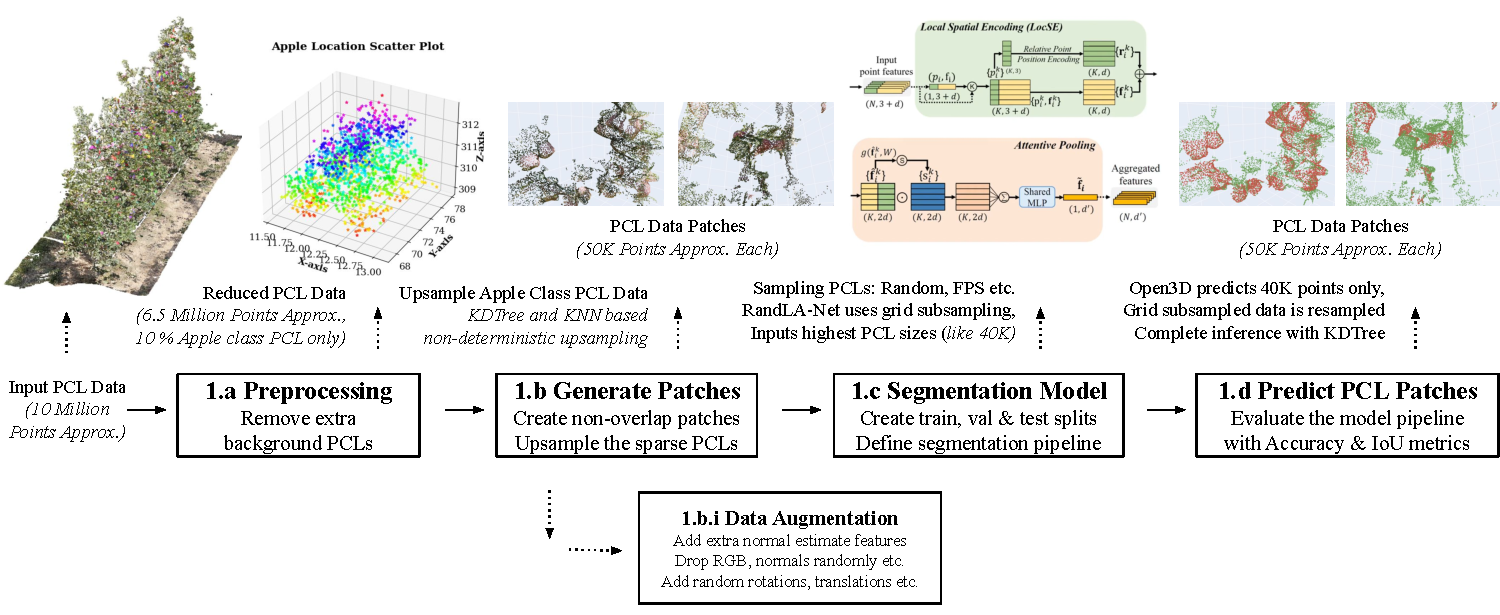
\includegraphics[width=0.95\textwidth]{point-cloud-data-processing-pipeline.pdf}
    \caption{The point cloud segmentation pipeline for processing large scale agriculture datasets.}
    \label{fig:pipeline}
\end{figure}


For robust model training, the training pipeline can be augmented with additional normal estimate features, random rotations and translations, and random RGB or normal feature estimate data drops, like specified in PointNext model training.
And, for segmentation model training the pipeline splits the data patches in train, validation, and test splits.
For the experiments, we used the RandLA-Net implementation from Open3D-ML package which inputs approximately 40K data points for every patch after grid subsampling, and makes predictions on those 40k data points.
At the complete point cloud inference stage for the patches, the inference made on these 40K data points is copied onto other previously subsampled nearest points by reusing the same KDTree that was utilized in the grid subsampling stage.
This inference for patches in the pipeline is a parallelizable operation which can make much faster predictions for large point clouds.
Much similar to processing and segmenting super resolution 2D images, as a known drawback this pipeline produces inconsistencies in prediction at the patch boundaries for all classes present in the point cloud.
This problem to some extent can be mitigated by using overlapping patches for training and inference, and further including confidence based probabilistic inference to classify a given point cloud data point.


\iffalse
\section{Experiment}
With the provided context, the thesis would be roughly structured as follows:
\subsection{Methodology Description}
\begin{itemize}
  \item \textbf{Abstract \& Introduction:} This section will highlight thesis topic relevance \& scope.
  \item \textbf{Related Literature:} Description of previous research work, and basic terminologies.
  \item \textbf{Mathematical Formulation:} This section will formally introduce our approach details.
  \item \textbf{Implementation Components:} This section will elaborate on all the system module details.
  \item \textbf{Methodology:} Comprise of scalability, robustness \& novelty experiment details.
  \item \textbf{Result Evaluation:} Comprise of RL evaluation metrics, SOTA comparisons \& visualizations.
  \item \textbf{Discussion \& Conclusion:} Comprise of limitation analysis, approach successes \& future work.
\end{itemize}
\subsection{Results and Discussion}
With the provided context, the thesis deliverable plan is structured as follows:
\fi


\section{Conclusion}


In this study we summarize multiple approaches from traditional image processing ones to the ones using modern deep learning models. \footnote{ Bibliography papers available at the repository \href{https://github.com/arana-initiatives/ai-portfolio-bibliography}{github.com/arana-initiatives/ai-portfolio-bibliography}.}
We also explore utilization of Mask R-CNN network on image data for generating segmentation masks for Fuji apples dataset.
And, further utilization of this post-processing techniques to generate segmented 3D point clouds.
This approach also counts apple instances and performs size estimation with a very high degree of accuracy.
Second, we explore approaches that can process agriculture point clouds, and their capacity to analyze large point cloud data.
And, we further analyze the most suitable RandLA-Net network in more detail which easily processes large point clouds, and we also address its limitations as well.
Finally, we propose a patch generation based solution for processing pipeline for 3D datasets which can be used to process large point cloud agriculture data directly.
And, in our practical experimentation we implement this data processing pipeline, and summarize challenges associated with building a realistic solution for large scale 3D data processing.


\bibliographystyle{acm}
\bibliography{main}


\end{document}`
